\section{Thuyết minh đề tài}
\subsection{Tên đề tài, thời gian thực hiện, tổng kinh phí}
\begin{quote}
-\textbf{Tên đề tài:} Hệ thống khuyến nghị khóa học cho dữ liệu MOOCCubeX\\
-\textbf{Thời gian thực hiện:} 8 tuần \\
-\textbf{Tổng kinh phí dự kiến:} 6.000.000đ (Việt Nam Đồng)\\
\end{quote}
\subsection{Nhóm thực hiện:}
\begin{center}
\begin{tabular}{|| m{10em}  m{5em}  m{6em}||} 
 \hline
 Tên & MSSV & Vai trò \\ [0.5ex] 
 \hline\hline
 Nguyễn Hữu Nam & 22520917 & Chủ nhiệm  \\ 
 \hline
 Nguyễn Khánh & 22520641 & Nhân lực \\
 \hline
 Võ Đình Khánh & 22520659 & Nhân lực \\
 \hline
 Bùi Hồng Sơn & 22521246 & Nhân lực \\
 \hline
 Nguyễn Minh Sơn & 22521254 & Nhân lực\\ [1ex] 
 \hline
\end{tabular}
\end{center}
\subsection{Mô tả đề tài}
\subsubsection{Giới thiệu về bài toán}
Khai phá dữ liệu, đặc biệt là dữ liệu lớn, đã trở thành một lĩnh vực nghiên cứu quan trọng và thu hút sự quan tâm của các nhà khoa học trong những năm gần đây. Các ứng dụng của khai phá dữ liệu rất đa dạng, được triển khai trong nhiều lĩnh vực như kinh doanh, giáo dục, y tế, tài chính, và ngân hàng. Đặc biệt, khai phá dữ liệu trong giáo dục, cụ thể là khai phá dữ liệu lớn, đang là chủ đề thu hút nhiều nghiên cứu nhờ vào tính ứng dụng cao và tiềm năng cải thiện chất lượng giáo dục\\
\\
Trong bối cảnh giáo dục trực tuyến hiện nay, người học phải tự chủ động và có tinh thần tự giác cao do số lượng môn học đa dạng thuộc nhiều lĩnh vực khác nhau. Họ cần phải phân bổ thời gian học tập hợp lý cho từng nhóm môn học, nhằm bổ sung và nâng cao kiến thức chuyên ngành cần thiết. Tuy nhiên, các nền tảng học tập trực tuyến thường không có ràng buộc cụ thể về thời gian và điểm số, dẫn đến tình trạng nhiều khóa học không được hoàn thành đúng thời hạn, thậm chí bị bỏ dở do người học mất hứng thú.\\
\\
Vì vậy, công tác cố vấn học tập trên các nền tảng trực tuyến trở nên vô cùng quan trọng để giúp người học cải thiện hiệu suất học tập và gợi ý các khóa học phù hợp với nhu cầu cá nhân. Đây là một bài toán thuộc lĩnh vực khai phá dữ liệu, đặc biệt là với số lượng lớn dữ liệu liên quan đến người học và hành vi học tập của họ trong quá trình tham gia các nền tảng học tập trực tuyến. Việc nghiên cứu và xây dựng hệ thống khuyến nghị khóa học sẽ góp phần quan trọng vào việc cá nhân hóa trải nghiệm học tập, hỗ trợ người dùng lựa chọn các khóa học phù hợp với nhu cầu và mục tiêu học tập của mình.\\
\\
\textbf{Định nghĩa và ngữ cảnh bài toán:}\\
Trong bối cảnh các nền tảng học tập trực tuyến, người học thường gặp khó khăn trong việc lựa chọn khóa học phù hợp. Điều này đặt ra nhu cầu xây dựng một hệ thống khuyến nghị giúp cá nhân hóa quá trình học tập của từng người. Sinh viên từ nhiều trường đại học khác nhau tại Trung Quốc phải đối mặt với khó khăn khi lựa chọn khóa học phù hợp trong một môi trường học tập trực tuyến quy mô lớn với hơn 4,216 khóa học và dữ liệu học tập phong phú, bài toán được đặt ra để giải quyết vấn đề này, tiết kiệm thời gian, đưa ra khoá học phù hợp với mục tiêu cá nhân của học sinh sinh viên. Cụ thể, bài toán được định nghĩa với đầu vào và đầu ra như sau: 
\begin{itemize}
    \item \textbf{Input:} Nguồn dữ liệu lớn từ các nền tảng học tập trực tuyến, bao gồm thông tin về người học, thông tin khóa học, và dữ liệu về các hoạt động học tập của người dùng.
    \item \textbf{Output:} Đề xuất top k khóa học phù hợp nhất với người dùng (trong đó k thuộc N* và trong đồ án này, k = 10 )
\end{itemize}

\subsubsection{Ứng dụng}
Bài toán khuyến nghị khóa học cho các nền tảng học tập trực tuyến có nhiều ứng dụng thực tiễn quan trọng, góp phần nâng cao chất lượng giáo dục và cá nhân hóa trải nghiệm học tập của người dùng. Dưới đây là một số ứng dụng nổi bật của bài toán:
\begin{itemize}
    \item Cá nhân hóa quá trình học tập: Hệ thống khuyến nghị giúp người học tìm kiếm và lựa chọn các khóa học phù hợp với nhu cầu và trình độ của mình. Dựa trên thông tin cá nhân và hành vi học tập, hệ thống có thể đề xuất những khóa học đáp ứng mục tiêu học tập cụ thể, giúp cá nhân hóa lộ trình học tập cho từng người dùng
    \item Tăng tỷ lệ hoàn thành khóa học: Nhiều người học trực tuyến gặp khó khăn trong việc duy trì động lực học tập, dẫn đến việc bỏ dở các khóa học. Hệ thống khuyến nghị có thể gợi ý các khóa học phù hợp hơn, giúp người học dễ dàng tiếp cận nội dung mà họ thực sự quan tâm, từ đó tăng tỷ lệ hoàn thành khóa học
    \item Tối ưu hóa lộ trình học tập: Dựa tren dữ liệu về các khóa học đã hoàn thành và kỹ năng hiện tại của người học, hệ thống có thể đề xuất các khóa học kế tiếp theo lộ trình hợp lý. Điều này giúp người học xây dựng lộ trình phát triển kỹ năng một cách hệ thống và hiệu quả
    \item Ứng dụng trong đào tạo doanh nghiệp: Đối với các doanh nghiệp, hệ thống khuyến nghị khóa học có thể được sử dụng để xây dựng chương trình đào tạo nhân viên, gợi ý các khóa học nâng cao kỹ năng phù hợp với từng nhân viên dựa trên vị trí công việc và kế hoạch phát triển nghề nghiệp
    \item Nâng cao hiệu quả sử dụng tài nguyên học tập: Hệ thống giúp người học tiếp cận đúng khóa học phù, tránh lãng phí thời gian và tài nguyên vào các khóa học không phù hợp. Điều này góp phần tối ưu hóa việc sử dụng các tài nguyên giáo dục trên nền tảng trực tuyến.
\end{itemize}
Nhờ vào các ứng dụng trên, hệ thống khuyến nghị khóa học không chỉ mang lại lợi ích cho người dùng mà còn giúp các nền tảng trực tuyến phát triển mạnh mẽ hơn, đáp ứng tốt hơn nhu cầu ngày càng đa dạng của người dùng.
\subsubsection{Khó khăn và thách thức}
\textbf{Chất lượng và sự đa dạng của dữ liệu:} Dữ liệu MOOCCubeX có thể không đồng nhất hoặc không đầy đủ cho tất cả người học, gây khó khăn trong việc phân tích hành vi và đặc điểm người dùng. Ví dụ, một số người dùng có thể chỉ đăng ký một số ít khóa học trong khi một số khác lại đăng ký quá nhiều hoặc không cung cấp đầy đủ thông tin cá nhân, thiếu đi thời gian hoàn thành khóa học cũng như đánh giá khóa học.\\
\\
\textbf{Thao tác với dữ liệu lớn:} Dữ liệu MOOCCubeX bao gồm hàng triệu người dùng và hàng nghìn khóa học cùng với đó là rất nhiều dữ liệu liên quan khác, hành vi xem video của người dùng, hành vi trả lời câu hỏi kiểm tra, bình luận... Việc xử lý và phân tích khối lượng dữ liệu lớn này đòi hỏi khả năng tính toán mạnh mẽ, cũng như tối ưu hóa thuật toán và cách xử lý dữ liệu để tránh các vấn đề về tài nguyên tính toán và thời gian thực thi.\\
\\
\textbf{Lựa chọn các đặc trưng quan trọng và cần thiết:} Bộ dữ liệu MOOCCubeX cung cấp nhiều thông tin chi tiết về tương tác của người dùng với các khóa học. Khó khăn trong việc lựa chọn dữ liệu thực sự cần thiết và các đặc trưng quan trọng. Đồng thời cũng phải chú trọng về phần tài nguyên và thời gian xử lý cũng làm giới hạn đi số lượng đặc trưng có thể chọn được.\\
\\
\textbf{Đánh giá mô hình:} Việc đánh giá mô hình khuyến nghị khóa học là một thách thức khi không có dữ liệu rõ ràng về mức độ hài lòng của người học. Ở đây chúng ta chỉ đánh giá được xem liệu rằng mô hình có dự đoán được khóa học người dùng sẽ đăng ký tiếp theo hay không. Điều này làm giảm đi phần nào tính chính xác và tổng quát của hệ khuyến nghị.
\subsubsection{Các dự án liên quan cùng lĩnh vực}
\textbf{Matrix Factorization:} Dựa trên việc tạo ma trận user-item và tìm mối tương quan tiềm ẩn bên trong (Koren, Y., Bell, R., \& Volinsky, C. (2009). Matrix Factorization Techniques for Recommender Systems).\\
\\
\textbf{Collaborative Filtering:}  Sử dụng các phương pháp như User-User hoặc Item-Item để tạo ra các gợi ý dựa trên sự tương đồng giữa user hoặc giữa các item (Su, X., \& Khoshgoftaar, T. M. (2009). A Survey of Collaborative Filtering Techniques).\\
\\
\textbf{Content-Based Filtering:} Trích xuất feature của item sau đó gợi ý dựa trên các item trước đó (Content-based Recommender Systems: State of the Art and Trends).\\
\\
\textbf{Hybrid Recommender Systems:} Kết hợp giữa Collaborative Filtering và Content-Based Filtering. (Burke, R. (2002). Hybrid Recommender Systems: Survey and Experiments).\\
\\
\textbf{Graph-Based Recommender Systems:} Dựa trên đồ thị từ dữ liệu người dùng và khóa học, sử dụng các thuật toán như Random Walk hoặc PageRank để khám phá các kết nối giữa chúng. (Graph Based Recommendations: From Data Representation to Feature Extraction and Application).\\
\\
\textbf{Neural Collaborative Filtering:} Giải quyết vấn đề tuyến tính của phương pháp Matrix Factorization thông qua việc áp dụng cấu trúc Deep Learning (He, X., Liao, L., Zhang, H., Nie, L., \& Hu, X. (2017). Neural Collaborative Filtering).
\subsection{Tổng quan}
\subsubsection{Ý tưởng và kế hoạch triển khai}
Hệ thống khuyến nghị khóa học được xây dựng nhằm gợi ý các khóa học phù hợp cho từng người dùng dựa trên dữ liệu hành vi và thông tin cá nhân của họ. Cụ thể, hệ thống sẽ sử dụng các kỹ thuật học máy như lọc cộng tác (Collaborative Filtering), lọc nội dung (Content-based Filtering) hoặc các mô hình học sâu (Deep Learning) để đưa ra khuyến nghị. Kế hoạch triển khai bao gồm các bước:
\begin{itemize}
    \item Tiền xử lý dữ liệu từ bộ MOOCCubeX.
    \item Xây dựng mô hình dự đoán khóa học dựa trên các thuật toán phù hợp.
    \item Đánh giá và tối ưu mô hình dựa trên các chỉ số đánh giá (metrics) như độ chính xác (accuracy), F1-score, và độ hài lòng của người dùng.
    \item Xây dựng hệ thống điện toán đám mây để huấn luyện mô hình và giao diện ứng dụng.
    \item Phát triển giao diện ứng dụng cho người dùng cuối nhằm hiển thị các khóa học được gợi ý.
\end{itemize}
\subsubsection{Tính cấp thiết}
Trong bối cảnh giáo dục trực tuyến ngày càng phát triển, số lượng khóa học và nội dung học tập đang tăng lên một cách nhanh chóng. Các nền tảng học tập trực tuyến như Coursera, edX hay các hệ thống giáo dục mở thường cung cấp hàng ngàn khóa học từ nhiều lĩnh vực khác nhau. Người dùng thường gặp khó khăn khi phải lựa chọn khóa học phù hợp với nhu cầu cá nhân. Vấn đề này dẫn đến một số hệ quả sau:
\begin{itemize}
    \item Quá tải thông tin (Information Overload)
    \item Tăng tỉ lệ bỏ học (High Dropout Rate)
    \item Nhu cầu cá nhân hóa trải nghiệm học tập (Personalized Learning)
    \item Giúp doanh nghiệp tối ưu hóa chiến lược cung cấp khóa học
    \item Cạnh tranh trong thị trường giáo dục trực tuyến
\end{itemize}
Vì vậy, việc xây dựng hệ thống khuyến nghị khóa học là cần thiết để giúp người học tìm kiếm, chọn lọc và theo đuổi những khóa học phù hợp một cách dễ dàng hơn, đồng thời mang lại giá trị to lớn cho các doanh nghiệp giáo dục trực tuyến.
\subsubsection{Tính mới}
Mặc dù có nhiều hệ thống khuyến nghị đã được phát triển, việc áp dụng các mô hình tiên tiến như mô hình học sâu hoặc kết hợp nhiều phương pháp khác nhau trên bộ dữ liệu cụ thể như MOOCCubeX vẫn là một vấn đề mới. Bộ dữ liệu MOOCCubeX chứa các thông tin đặc thù về các khóa học trực tuyến, tạo điều kiện cho việc thử nghiệm các kỹ thuật và thuật toán tiên tiến để cải thiện khả năng khuyến nghị.
\subsection{Mục tiêu đề tài}
\subsubsection{Mục tiêu về đồ án}
\begin{itemize}
    \item Xây dựng một hệ thống khuyến nghị khóa học với các chỉ số đánh giá chất lượng như độ chính xác, F1-score đạt yêu cầu (>80%).
    \item Sử dụng bộ dữ liệu MOOCCubeX để huấn luyện và kiểm tra hệ thống, đảm bảo hệ thống hoạt động tốt với dữ liệu thực tế.
    \item Đưa ra báo cáo chi tiết về các thuật toán, mô hình đã sử dụng và kết quả đạt được. Ngoài ra, cần phân tích mức độ hiệu quả của các mô hình khác nhau để tìm ra phương pháp tối ưu nhất.
\end{itemize}
\subsubsection{Mục tiêu về doanh nghiệp}
Hệ thống khuyến nghị có tiềm năng ứng dụng trong các nền tảng học trực tuyến, giúp nâng cao trải nghiệm của người dùng và tăng mức độ hài lòng của họ. Điều này có thể dẫn đến việc tăng tỉ lệ giữ chân người dùng (user retention) và thu hút nhiều học viên mới, đồng thời tối ưu hóa nguồn lực và chi phí quảng bá các khóa học không phù hợp.
\subsubsection{Mục tiêu về sản phẩm}
Phát triển một ứng dụng có giao diện thân thiện với người dùng, cho phép học viên dễ dàng nhận được các khóa học phù hợp. Sản phẩm cần tích hợp dễ dàng với các nền tảng học trực tuyến hiện có và có khả năng mở rộng để hỗ trợ nhiều người dùng đồng thời mà không ảnh hưởng đến hiệu suất hệ thống.
\subsection{Input - Output}
\begin{itemize}
    \item \textbf{Input:} Nguồn dữ liệu lớn trong các nền tảng học tập trực tuyến: Thông tin người học, thông tin khóa học, hoạt động học tập của người dùng.
    \item \textbf{Output:} Đề xuất top k các khóa học phù hợp nhất với người dùng.
\end{itemize}
\begin{figure}[h]
    \centering
    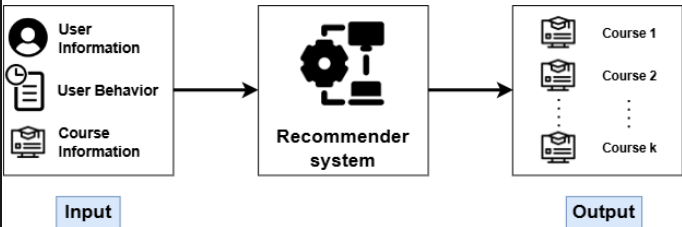
\includegraphics[width=0.75\linewidth]{image/55.png}
\end{figure}
\subsection{Nội dung bài toán triển khai}
\subsubsection{Nội dung 1}
\textbf{Mục tiêu 1:} Tiền xử lý cho các bảng dữ liệu trong bộ dữ liệu MOOCCubeX phục vụ nhiệm vụ Khuyến nghị khóa học cho người dùng.\\
\textbf{Phương pháp 1:}
\begin{itemize}
    \item Dịch bảng dữ liệu (Data translation)
    \item Làm sạch dữ liệu (Data Cleaning)
    \item Chuẩn hóa và chuẩn hóa dữ liệu (Normalization and Standardization)
    \item Mã hóa dữ liệu (Data Encoding)
    \item Tạo và chọn đặc trưng (Feature Engineering \& Feature Selection)
    \item Chia tập dữ liệu (Splitting the Data)
\end{itemize}
\subsubsection{Nội dung 2}
\textbf{Mục tiêu 2:} Xây dựng các mô hình học sâu tốt nhất với nhiệm vụ Khuyến nghị khóa học cho người dùng.\\
\textbf{Phương pháp 2:}\\
\textbf{1) KNN (K-Nearest Neighbors)}
    \begin{itemize}
        \item Đặc điểm: Dựa trên việc tìm kiếm các điểm lân cận gần nhất trong không gian đặc trưng để đưa ra dự đoán.
        \item Ưu điểm: Đơn giản, dễ hiểu, không cần phải huấn luyện mô hình.
        \item Nhược điểm: Hiệu suất kém với dữ liệu lớn và phân tán, khó mở rộng.
    \end{itemize}\\
\textbf{2) BERT4Rec}
\begin{itemize}
    \item Đặc điểm: Mô hình BERT (Bidirectional Encoder Representations from Transformers) được điều chỉnh cho hệ khuyến nghị tuần tự.
    \item Ưu điểm: Hiểu được ngữ cảnh tốt hơn nhờ việc mã hoá hai chiều, mạnh trong việc dự đoán dựa trên trình tự.
    \item Nhược điểm: Yêu cầu tính toán lớn, khó mở rộng với dữ liệu rất lớn.
\end{itemize}\\
\textbf{3) Neural Factorization Machines (NFM)}
\begin{itemize}
    \item Đặc điểm: Kết hợp mô hình Factorization Machines với mạng nơ-ron để học các tương tác phi tuyến giữa các đối tượng.
    \item Ưu điểm: Tốt hơn so với Factorization Machines trong việc nắm bắt các tương tác phức tạp.
    \item Nhược điểm: Cần nhiều tài nguyên tính toán hơn.
\end{itemize}

\textbf{Sản phẩm 2:} Mô hình học sâu tốt nhất được lựa chọn khi huấn luyện trên bộ dữ liệu MOOCCubeX với nhiệm vụ Khuyến nghị khóa học.\\
\textbf{* Các metric phù hợp với hệ khuyến nghị:}\\
\textbf{Precision \& Recall}
\begin{itemize}
    \item Precision đo lường phần trăm các gợi ý đúng trên tổng các gợi ý được đưa ra.
    \item Recall đo lường phần trăm các gợi ý đúng so với tổng số gợi ý có thể đưa ra (trong số các mặt hàng mà người dùng quan tâm).
    \item Giải thích: Precision và Recall giúp cân bằng giữa việc đưa ra đúng những gợi ý chất lượng (precision cao) và khả năng bao phủ đầy đủ các gợi ý mà người dùng có thể quan tâm (recall cao).
\end{itemize}\\
\textbf{NDCG (Normalized Discounted Cumulative Gain)}
\begin{itemize}
    \item Đặc điểm: Đánh giá mức độ phù hợp của các gợi ý, ưu tiên những gợi ý đúng nằm ở các vị trí đầu tiên trong danh sách.
    \item Giải thích: Phù hợp cho hệ khuyến nghị khi thứ tự của các gợi ý là quan trọng, giúp tối ưu hoá trải nghiệm người dùng khi họ thường chú ý tới các mục đầu tiên.
\end{itemize}\\
\textbf{AUC (Area Under Curve)}
\begin{itemize}
    \item Đặc điểm: Đo lường mức độ phân biệt giữa các mặt hàng ưa thích và không ưa thích dựa trên xác suất dự đoán.
    \item Giải thích: AUC phù hợp cho việc đánh giá khả năng của mô hình trong việc xếp hạng chính xác các mặt hàng mà người dùng quan tâm.
\end{itemize}
\subsubsection{Nội dung 3}
\textbf{Mục tiêu 3:} Tìm hiểu và lựa chọn nền tảng đám mây phù hợp cho lưu trữ, xử lý dữ liệu lớn (Microsoft Azure) cũng như xây dựng và huấn luyện mô hình học máy (Microsoft Azure, Kaggle).\\
\textbf{Phương pháp 3:}
\begin{itemize}
    \item Tận dụng các dịch vụ mà Microsoft Azure cung cấp cho việc lưu trữ và xử lý dữ liệu lớn: Azure Blob Storage, Azure Data Factory, Azure Data Lake Storage, Azure Databricks cùng các dịch vụ từ MS Azure và Kaggle cho quá trình xây dựng và huấn luyện mô hình học máy: Azure Machine Learning.
    \item Xây dựng được quy trình Big Data Architecture, từ bước Ingest, Process, Store đến bước Enrich và Serve.
    \item Các mô hình máy học được lưu trữ đầy đủ thông số sau quá trình thực nghiệm, phục vụ cho việc phát triển thành các ứng dụng thực tế cho nhiệm vụ khuyến nghị khóa học.
\end{itemize}
\begin{figure}[h]
    \centering
    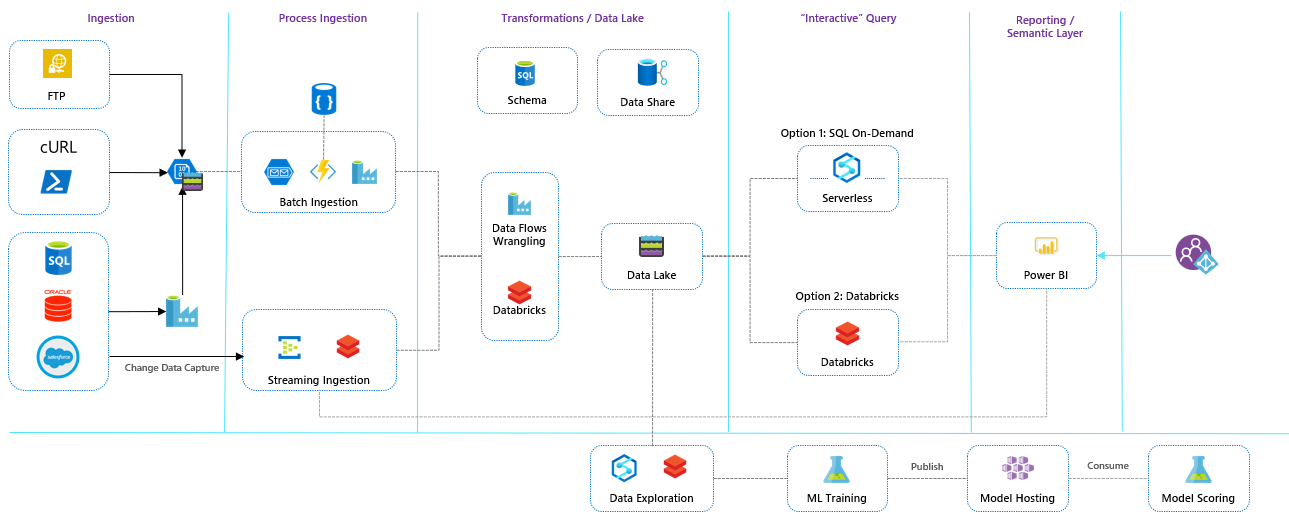
\includegraphics[width=0.75\linewidth]{image/56.png}
    \caption{Kiến trúc mẫu về việc xây dựng hệ thống sử dụng Machine Learning với Azure}
\end{figure}
\textbf{Sản phẩm 3:} Xây dựng thành công Big Data Architecture, Các mô hình máy học được lưu trữ đầy đủ thông số sau quá trình thực nghiệm, phục vụ cho việc phát triển thành các ứng dụng thực tế cho nhiệm vụ khuyến nghị khóa học.
\subsubsection{Nội dung 4}
\textbf{Mục tiêu 4:} Xây dựng ứng dụng Website để phục vụ việc tương tác giữa người
dùng và Hệ thống khuyến nghị.\\
\textbf{Phương pháp 4:} Sau khi thu được pretrained của mô hình học sâu tốt nhất được huấn luyện trên bộ dữ liệu MOOCCubeX trên nhiệm vụ Khuyến nghị các khóa học cho học viên. Sau đó sử dụng PostgreSQL (backend), React (front-end) và SQL để triển khai website. Kết quả thu được một ứng dụng Website trực quan, dễ dàng sử dụng, cho phép người dùng nhập vào các khóa học đã học, trả về tập gồm top-k các khóa học được hệ thống khuyến nghị.\\
\textbf{Sản phẩm 4:} Website tương tác với người dùng có chức năng khuyến nghị khoá học khi tìm khoá học mới, trả về tập gồm top-k các khóa học được hệ thống khuyến nghị.
